\subsection{Prostate anatomy}\label{section:intro:anatomy}

The prostate is an exocrine gland of the male reproductive system having an
inverted pyramidal shape, which is located below the bladder and in front of
the rectum as shown in \acs{fig}\,\ref{fig:prostatelocation}.
It measures approximately \SI{3}{\cm} in height by \SI{2.5}{\cm} in depth and
its weight is estimated from \SIrange{7}{16}{\gram} for an
adult~\cite{Leissner1979}.
The prostate size increases at two distinct stages during physical development:
initially at puberty to reach its normal size, then again after 60 years of age
leading to \ac{bph}~\cite{Parfait2010}.

A zonal classification of the prostate has been suggested by
\citeauthor{McNeal1981}~\cite{McNeal1981}, as depicted in
\acs{fig}\,\ref{fig:anatomyProstateZone}.
Subsequently, this categorization has been widely accepted in the
literature~\cite{Hricak1987,Villers1991,Coakley2000,Parfait2010} and is used
during all medical examinations (e.g., biopsy, \ac{mri} screening).
The classification is based on dividing the gland into 3 distinct regions: (i)
the \ac{cz} accounting for \SIrange{20}{25}{\percent} of the whole prostate
gland, (ii) the \ac{tz} standing for \SI{5}{\percent}, and (iii) the \ac{pz}
representing the \SI{70}{\percent}.
In \ac{mri} images, tissues of \ac{cz} and \ac{tz} are difficult to distinguish
and are usually merged into a common region, denominated \ac{cg}.
As part of this classification, the prostate is divided into 3 longitudinal
portions depicted in \acs{fig}\,\ref{fig:anatomyProstateSagittal}: (i) base,
(ii) median gland, and (iii) apex.

\subsection{Prostate carcinoma}

\begin{figure}
  \centering
  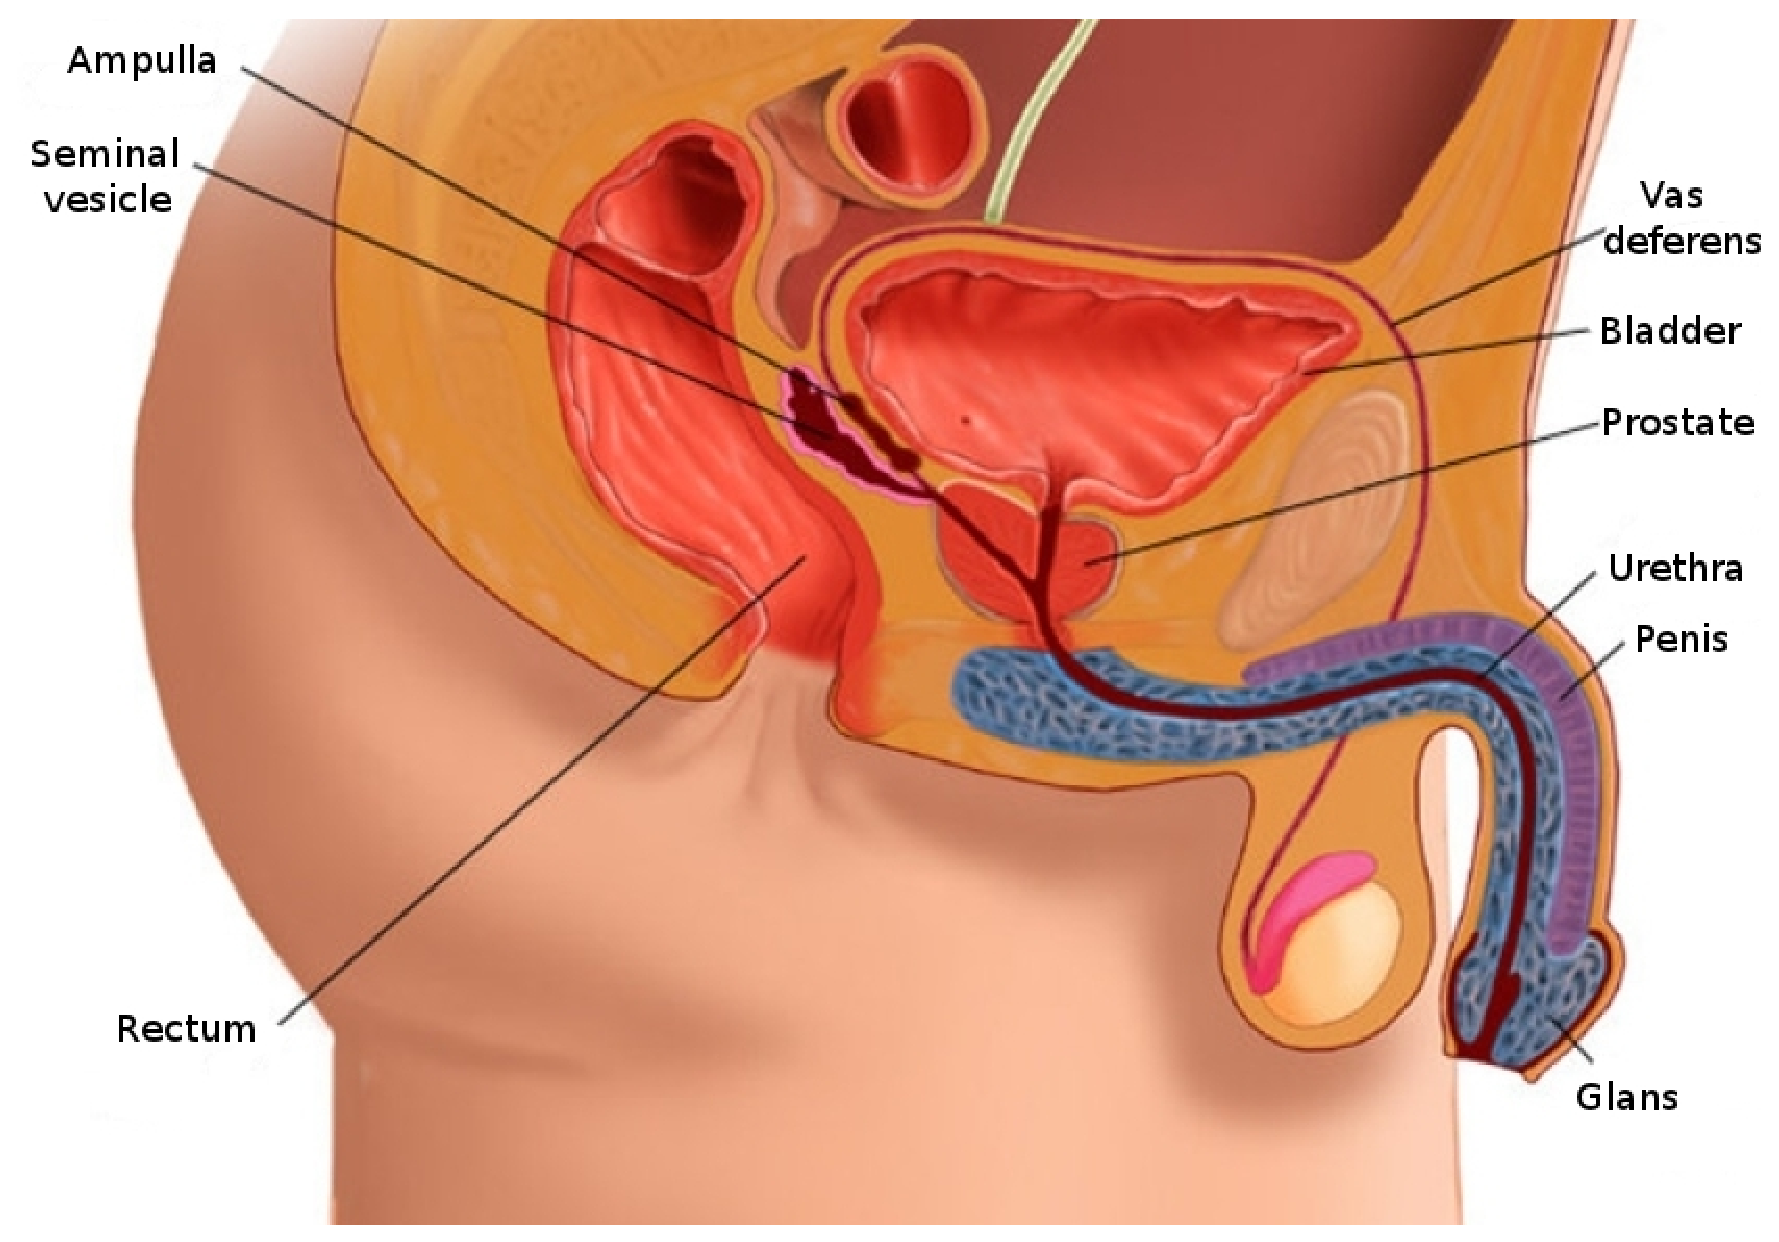
\includegraphics[height=0.25\textheight]{1_introduction/figures/anatomy/prostate2D.eps}
  \caption[Sagittal anatomy of prostate.]{Sagittal anatomy scheme of the male
    reproductive system (copyright by~\cite{Geckomedia2011}).}
  \label{fig:prostatelocation}
\end{figure}

\begin{figure}
  \centering
  \hspace*{\fill}
  \subfloat[Transverse anatomy of the prostate.]{
    \centering
    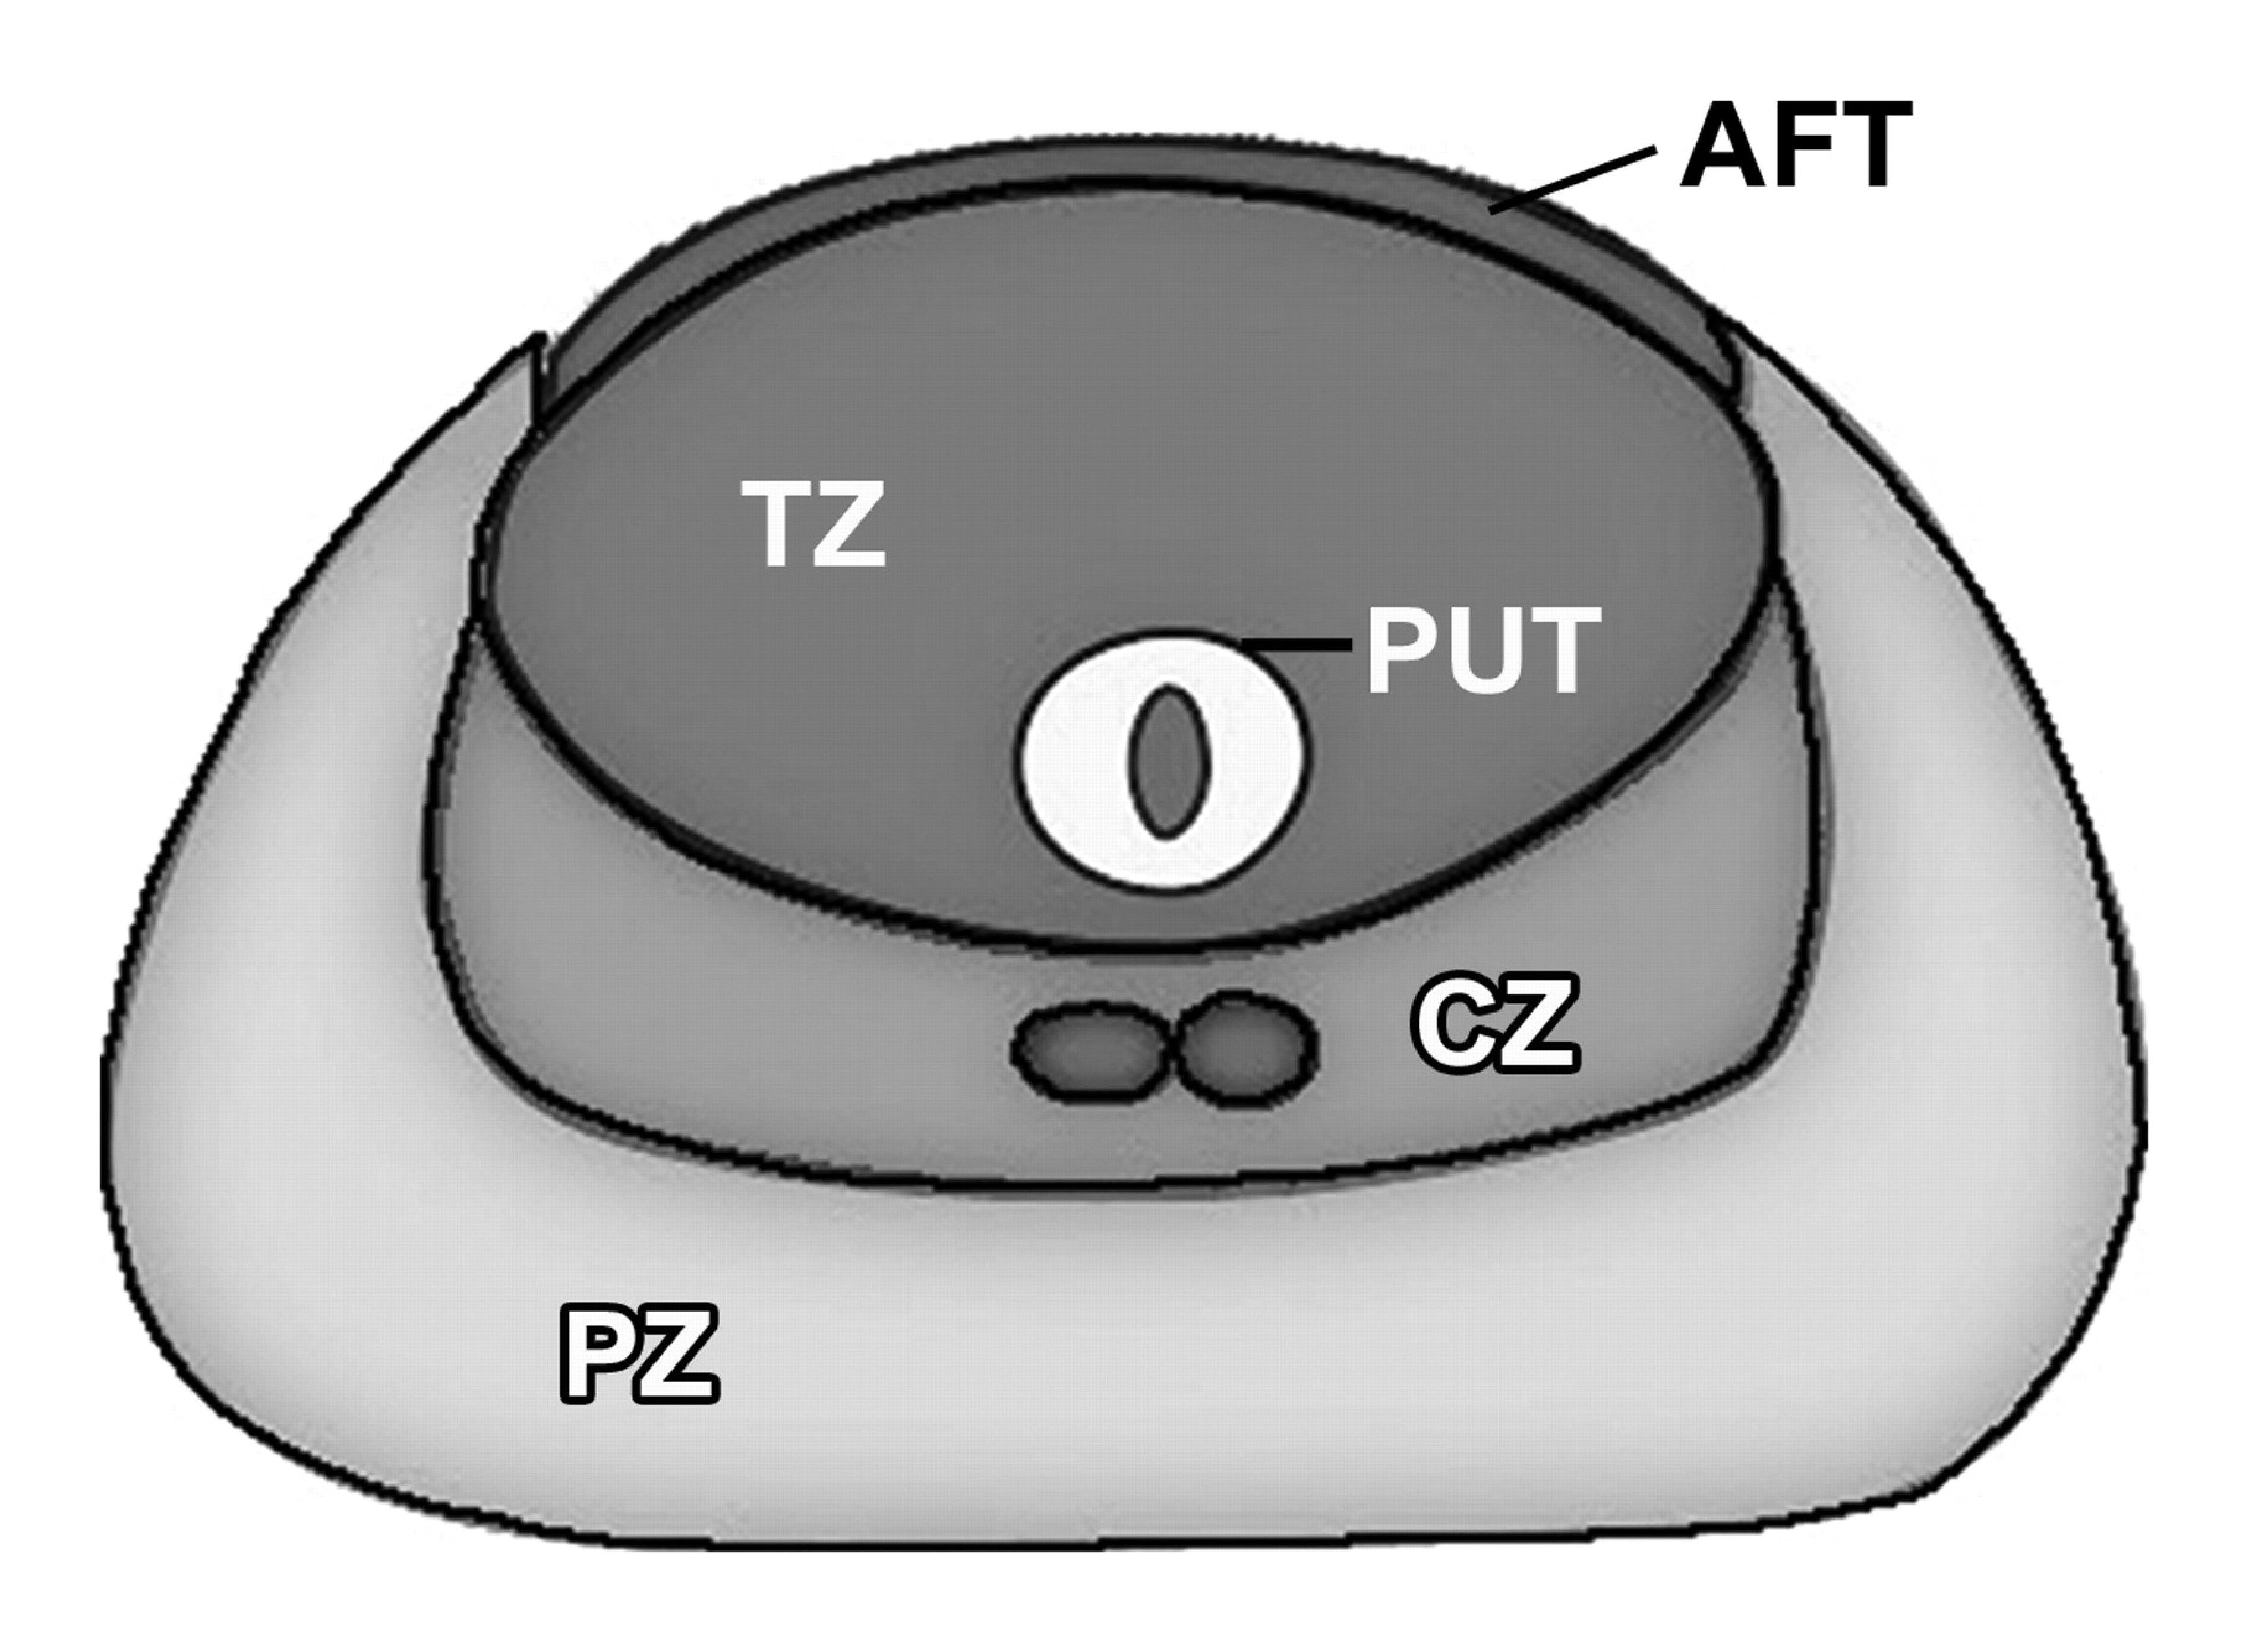
\includegraphics[height=0.15\textheight]{1_introduction/figures/anatomy/prostateTransverse.eps}
    \label{fig:anatomyProstateTransverse}}
  \hfill
  \subfloat[Sagittal anatomy of the prostate.]{
    \centering
    \includegraphics[height=0.23\textheight]{1_introduction/figures/anatomy/prostateSagital.eps}
    \label{fig:anatomyProstateSagittal}}\hspace*{\fill}
  \caption[Prostate anatomy.]{Prostate anatomy with division in different
    zones. \textit{AFT:} anterior fibromuscular tissue, \textit{CZ:} central
    zone, \textit{ED:} ejaculatory duct, \textit{NVB:} neurovascular bundle,
    \textit{PUT:} periurethral tissue, \textit{PZ:} peripheral zone,
    \textit{U:} urethra, \textit{TZ:} transitional zone, \textit{B:} base,
    \textit{M:} median, \textit{A:} apex (copyright by~\cite{Choi2007}).}
  \label{fig:anatomyProstateZone}
\end{figure}

Prostate cancer \ac{cap} has been reported on a worldwide scale to be the
second most frequently diagnosed cancer of men accounting for
\SI{13.6}{\percent}~\cite{Ferlay2010}.
Statistically, in 2008, the number of new diagnosed cases has been estimated to
be $899,000$ with no less than $258,100$ deaths~\cite{Ferlay2010}.
In United States, aside from skin cancer, \ac{cap} is declared to be the most
commonly diagnosed cancer among men, implying that approximately 1 in 6 men
will be diagnosed with \ac{cap} during their lifetime and 1 in 36 will die from
this disease, causing \ac{cap} to be the second most common cause of cancer
death among men~\cite{Siegel2013,Society2013}.

Despite active research to determine the causes of \ac{cap}, a fuzzy list of
risk factors has arisen~\cite{Society2010}.
The etiology has been linked to the following factors~\cite{Society2010}: (i)
family history~\cite{Giovannucci2007,Steinberg1990}, (ii) genetic
factors~\cite{Freedman2006,Amundadottir2006,Agalliu2009}, (iii)
race-ethnicity~\cite{Giovannucci2007,Hoffman2001}, (iv)
diet~\cite{Giovannucci2007,Ma2009,Alexander2010}, and (v)
obesity~\cite{Giovannucci2007,Rodriguez2007}.
This list of risk factors alone cannot be used to diagnose \ac{cap} and in this
way, screening enables early detection and treatment.

\ac{cap} growth is characterized by two main types of
evolution~\cite{Strum2005}: slow-growing tumours, accounting for up to
\SI{85}{\percent} of all \acp{cap}~\cite{Lu-Yao2009}, progress slowly and
usually stay confined to the prostate gland.
For such cases, treatment can be substituted with active surveillance.
In contrast, the second variant of \acp{cap} develops rapidly and metastasises
from prostate gland to other organs, primarily the bones~\cite{Oster2013}.
Bone metastases, being an incurable disease, significantly affects the
morbidity and mortality rate~\cite{Ye2007}.
Hence, the results of the surveillance have to be trustworthy in order to
distinguish aggressive from slow-growing \ac{cap}.

\ac{cap} is more likely to come into being in specific regions of the prostate.
In that respect, around \SIrange{70}{80}{\percent} of \acp{cap} originate in
\ac{pz} whereas \SIrange{10}{20}{\percent} in
\ac{tz}~\cite{Carrol1987,McNeal1988,Stamey1998}.
Only about \SI{5}{\percent} of \acp{cap} occur in
\ac{cz}~\cite{McNeal1988,Cohen2008}.
However, those cancers appear to be more aggressive and more likely to invade
other organs due to their locations~\cite{Cohen2008}.
